%versi 2 (8-10-2016)
\chapter{Landasan Teori}
\label{chap:teori}

Pada bab ini akan diuraikan teori-teori yang akan digunakan untuk pembangunan aplikasi ke analisis kota Bandung. Teori-teori tersebut adalah penjelasan tentang protokol HTTP, Penjelasan tentang \textit{JSOUP API}, Penjelasan tentang \textit{Google Direction API} dan teori JSON.

\section{Protokol HTTP}
\label{sec:protocolhttp} 

HTTP adalah protokol di balik World Wide Web. Dengan setiap transaksi web, HTTP dipanggil. HTTP adalah di balik setiap permintaan dokumen web atau grafis, setiap klik link hypertext, dan setiap penyerahan formulir. Web adalah tentang penyebaran informasi melalui Internet, dan HTTP adalah protokol yang digunakan untuk melakukannya.

\subsection{Transaksi HTTP}
\label{subsec:architecturehttp}

Berikut akan diilustrasikan transaksi web umum, menunjukkan HTTP yang dipertukarkan antara program \textit{client} dan \textit{program} server. \cite{wong2000http}:

\begin{itemize}
	\item berikut diberikan sebuah url : http:\/\/hypothetical.ora.com:80\/.
	\item Browser akan mengintepretasikan URL tersebut sebagai berikut :
			\begin{itemize}
				\item \(http:\/\/\) : menggunakan protokol HTTP.
				\item \(hypothetical.ora.com\) : menghubungi komputer melalui jaringan dengan hostname hypothetical.ora.com.
				\item \(:80\) : Terhubung ke komputer di port 80. Nomor port IP nomor dari 1 sampai 65535. Jika titik dua dan nomor port dihilangkan, nomor port diasumsikan nomor port \textit{default} HTTP, yang merupakan 80.
				\item \(\/\) : Apapun setelah nama host dan nomor port opsional dianggap sebagai jalan dokumen. Dalam ilustrasi ini, jalan dokumen adalah \/.
			\end{itemize}
			\item Pada ilustrasi ini browser menghubungkan ke hypothetical.ora.com pada port 80 menggunakan protokol HTTP. Pesan bahwa browser mengirimkan ke server adalah sebagai berikut:
			\begin{figure}[H]
				\centering		
				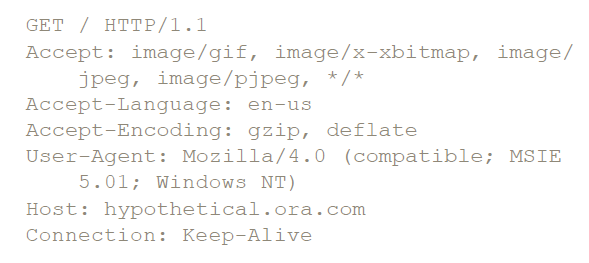
\includegraphics[scale=1]{Gambar/request.png}
				\caption[HTTP Request]{HTTP Request\cite{wong2000http}}
				\label{fig:httprequest}	
			\end{figure}
			\item 
\end{itemize}

\section{JSOUP API}
\label{sec:jsoupapi} 

\section{Google Direction API}
\label{subsec:googledirapi}

\section{JSON}
\label{sec:json}

JSON (JavaScript Object Notation) adalah format pertukaran data yang ringan, mudah dibaca dan ditulis oleh manusia, serta mudah diterjemahkan dan dibuat (generate) oleh komputer. Format ini dibuat berdasarkan bagian dari Bahasa Pemprograman JavaScript, Standar ECMA-262 Edisi ke-3 - Desember 1999. JSON merupakan format teks yang tidak bergantung pada bahasa pemprograman apapun karena menggunakan gaya bahasa yang umum digunakan oleh programmer keluarga C termasuk C, C++, C#, Java, JavaScript, Perl, Python dll. Oleh karena sifat-sifat tersebut, menjadikan JSON ideal sebagai bahasa pertukaran-data.

\subsection{Struktur JSON}
\label{subsec:stukturjson}
JSON terbuat dari dua struktur :
\begin{itemize}
	\item Kumpulan pasangan nama/nilai.
	\item Daftar nilai terurutkan (an ordered list of values).
\end{itemize} 

Struktur-struktur data ini disebut sebagai struktur data universal. Pada dasarnya, semua bahasa pemprograman moderen mendukung struktur data ini dalam bentuk yang sama maupun berlainan. Hal ini pantas disebut demikian karena format data mudah dipertukarkan dengan bahasa-bahasa pemprograman yang juga berdasarkan pada struktur data ini.
 
\subsection{Bentuk-Bentuk JSON}
\label{subsec:bentukjson}
\begin{itemize}
	\item Objek
	Objek adalah sepasang nama/nilai yang tidak terurutkan. Objek dimulai dengan { (kurung kurawal buka) dan diakhiri dengan } (kurung kurawal tutup). Setiap nama diikuti dengan : (titik dua) dan setiap pasangan nama atau nilai dipisahkan oleh , (koma).
	\begin{figure}[H]
		\centering		
		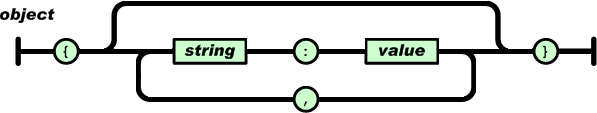
\includegraphics[scale=0.8]{Gambar/object.gif}
		\caption[JSON Object]{JSON Object}
		\label{fig:jsonobject}	
	\end{figure}
	\item \textit{Array}
	\textit{Array} adalah kumpulan nilai yang terurutkan. Larik dimulai dengan [ (kurung kotak buka) dan diakhiri dengan ] (kurung kotak tutup). Setiap nilai dipisahkan oleh , (koma).
	\begin{figure}[H]
		\centering		
		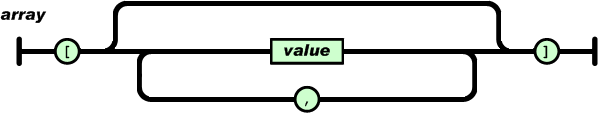
\includegraphics[scale=0.8]{Gambar/array.gif}
		\caption[JSON Object]{JSON Array}
		\label{fig:jsonarray}	
	\end{figure}
\end{itemize} 

\subsection{Value JSON}
\label{subsec:bentukjson}
Nilai(\textit{value})dapat berupa sebuah string dalam tanda kutip ganda, atau angka, atau true atau false atau null, atau sebuah objek atau sebuah larik. Struktur-struktur tersebut dapat disusun bertingkat.
\begin{figure}[H]
	\centering		
	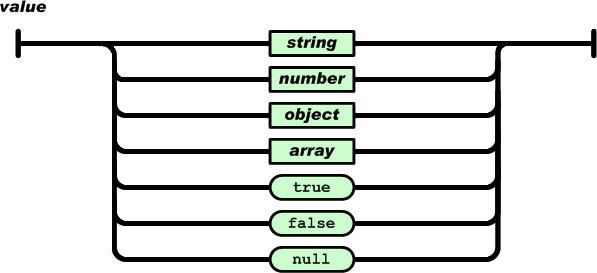
\includegraphics[scale=0.8]{Gambar/value.gif}
	\caption[Value]{Value}
	\label{fig:value}	
\end{figure}

\subsubsection{\textit{String}}
\label{subsubsec:string}
String adalah kumpulan dari nol atau lebih karakter Unicode, yang dibungkus dengan tanda kutip ganda. Di dalam string dapat digunakan backslash escapes "\" untuk membentuk karakter khusus. Sebuah karakter mewakili karakter tunggal pada string. String sangat mirip dengan string C atau Java.

\begin{figure}[H]
	\centering		
	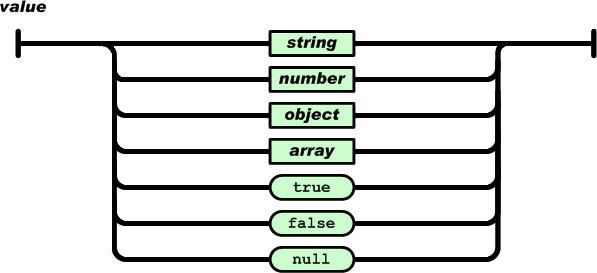
\includegraphics[scale=0.8]{Gambar/value.gif}
	\caption[String]{String}
	\label{fig:string}	
\end{figure}

\subsubsection{Angka}
\label{subsubsec:Angka}
Angka adalah sangat mirip dengan angka di C atau Java, kecuali format oktal dan heksadesimal tidak digunakan.
\begin{figure}[H]
	\centering		
	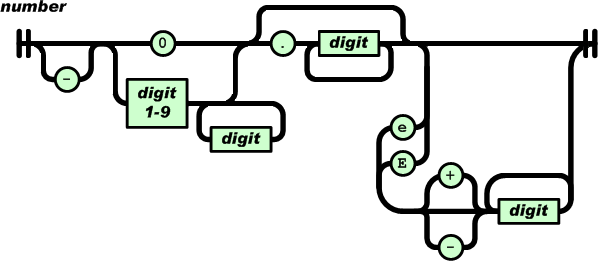
\includegraphics[scale=0.8]{Gambar/number.gif}
	\caption[Angka]{Angka}
	\label{fig:number}	
\end{figure}